\documentclass{article}
\usepackage{fullpage}
\usepackage{amsfonts}
\usepackage{amssymb}
\usepackage{amsmath}
\usepackage{hyperref}
\usepackage{graphicx}% Include figure files
\usepackage{epstopdf}
\usepackage{subfig}

%\usepackage{setspace}\doublespace
\author{Guojun Zhu}
\title{Narrow Feshbach Resonance}
\newcommand{\vk}{\ensuremath{\mathbf{k}}}
\newcommand{\vK}{\ensuremath{\mathbf{K}}}
\providecommand{\vr}{\ensuremath{\mathbf{r}}}
%\newcommand{\vec}[1]{\ensuremath{\mathbf{#1}}}

\newcommand{\gk}{\ensuremath{{g}(\mathbf{k})}}

\newcommand{\vp}{\ensuremath{\mathbf{p}}}
\newcommand{\gp}{\ensuremath{{g}(\mathbf{p})}}

\newcommand{\vq}{\ensuremath{\mathbf{q}}}

\newcommand{\Fo}{\ensuremath{\mathbf{F_0}}}


\newcommand{\E}{\ensuremath{\mathbf{E}}}
\newcommand{\A}{\ensuremath{\mathbf{A}}}
\newcommand{\J}{\ensuremath{\mathcal{J}}}

\newcommand{\ket}[1]{\ensuremath{\left|#1\right>}}
\newcommand{\bra}[1]{\ensuremath{\left<#1\right|}}

\newcommand{\twoe}{\ensuremath{2\epsilon_\vk-\E_1}}

\newcommand{\nth}[1]{\ensuremath{\frac{1}{#1}}}

\newcommand{\br}[1]{\ensuremath{\left(#1\right)}}
\newcommand{\mbr}[1]{\ensuremath{\left[#1\right]}}
\newcommand{\bbr}[1]{\ensuremath{\left\{#1\right\}}}


\newcommand{\tk}{\ensuremath{\tilde{k}}}

\newcommand{\kp}{\ensuremath{\ket{\Psi}}}

\newcommand{\av}[1]{\ensuremath{\bigl<{#1}\bigr>}}
\newcommand{\avs}[3] {\av{#1{\lvert{#2}\rvert}#3}}
\newcommand{\avv}[2][\nu] {\avs{#1}{#2}{#1}}
\newcommand{\avt}[2]{\av{{#1}|{#2}}}
\newcommand{\avtu}[1]{\av{T_\tau#1}}

\newcommand{\Bop}{\ensuremath{\mathbf{B_0^+}}}
\newcommand{\Bmp}{\ensuremath{\mathbf{B_m^+}}}
\newcommand{\Bnp}{\ensuremath{\mathbf{B_n^+}}}
\newcommand{\Bo}{\ensuremath{\mathbf{B_0}}}
\newcommand{\Bopn}{\ensuremath{\mathbf{{B_0^+}^n}}}
\newcommand{\Bon}{\ensuremath{\mathbf{{B_0}^n}}}


\newcommand{\zmatrix}{\ensuremath{\br{\begin{smallmatrix}0&0\\0&0\end{smallmatrix}}}}
\newcommand{\fmtrx}[4]{\ensuremath{\br{\begin{smallmatrix}#1&#2\\#3&#4\end{smallmatrix}}}}
\newcommand{\smtrx}[6]{\ensuremath{\br{\begin{smallmatrix}#1&#2\\#3&#4\\#5&#6\end{smallmatrix}}}}

\newcommand{\vz}{\ensuremath{v^{\beta\alpha}_{\vk,\vk}}}


\providecommand{\abs}[1]{\ensuremath{\lvert{#1}\rvert}}

\newcommand{\sg}[1][1]{\ensuremath{\sigma_\frac{#1}{2}}}

\newcommand{\rhof}{\ensuremath{\rho(\ef)}}
\newcommand{\omt}{\ensuremath{\tilde{\Omega}}}
\newcommand{\cht}{\ensuremath{\tilde{\chi_0}}}
\newcommand{\Atl}{\ensuremath{\abs{A}^{2l}}}
\newcommand{\ef}{\ensuremath{\epsilon_F}}

\newcommand{\lca}{\ensuremath{\ln\br{1+\frac{\cht}{\alpha}}}}

\newcommand{\com}[2]{\ensuremath{\mbr{#1,#2}}}
\newcommand{\D}{\ensuremath{\mathit{D}}}
\newcommand{\dg}{\ensuremath{\dagger}}
\newcommand{\nG}{\ensuremath{\hat{\mathcal{G}}^{-1}}}

\providecommand{\lvk}{\ensuremath{1/\vk_F}}
\providecommand{\hm}{\ensuremath{\frac{\hbar^2}}{2m}}
\providecommand{\pdiff}[2]{\ensuremath{\frac{\partial{#1}}{\partial{#2}}}}
\providecommand{\dpdiff}[2]{\ensuremath{\frac{\partial^2{#1}}{\partial{{#2}^2}}}}

\providecommand{\H}{\ensuremath{\mathcal{H}}}
\providecommand{\wt}[1]{\widetilde{#1}}

\providecommand{\eef}[1]{Eq. (\ref{#1})}

\providecommand{\sch}{{Schr\"{o}dinger }}

\providecommand{\sgn}{\ensuremath{\text{sgn}}}
\newcommand{\Arctg}{\ensuremath{\text{Arctg}}}

\providecommand{\comm}[1]{\textit{\scriptsize \uwave{(#1)}}}
\renewcommand{\emph}[1]{\textbf{#1}}
\begin{document}
\maketitle

%\tableofcontents
\numberwithin{equation}{section}
\section{}
 The full two-channel hamiltonian is
\begin{equation}\label{eq:uvw:hamiltonian}
\begin{split}
 H=&\sum_\vk\epsilon^a_\vk{}a^+_\vk{}a^{}_\vk+\sum_\vk\epsilon^b_\vk{}b^+_\vk{}b^{}_\vk+\sum_\vk\epsilon^c_\vk{}c^+_\vk{}c^{}_\vk\\
  &+\nth{2}\sum_{\vk\vk'}U_{\vk\vk'}a^+_\vk{}b^+_{-\vk}{}b^{}_{-\vk'}a^{}_{\vk'}
	+\nth{2}\sum_{\vk\vk'}V_{\vk\vk'}a^+_\vk{}c^+_{-\vk}{}c^{}_{-\vk'}a^{}_{\vk'}\\
 &+\nth{2}\sum_{\vk\vk'}Y_{\vk\vk'}a^+_\vk{}b^+_{-\vk}{}c^{}_{-\vk'}a^{}_{\vk'}
	+\nth{2}\sum_{\vk\vk'}Y^*_{\vk\vk'}a^+_{\vk'}{}c^+_{-\vk'}{}b^{}_{-\vk}a^{}_{\vk}
\end{split} 
\end{equation}
 We start from the ansatz as 
\begin{equation}\label{eq:ansatz}
 \ket{\Psi}=\prod_\vk\br{u_\vk+v_\vk{}a^\dg_\vk{}b^\dg_{-\vk}+w_\vk{}a^\dg_\vk{}c^\dg_{-\vk}}\ket{0}
\end{equation}
The free energy is 
\begin{equation}\label{eq:uvw:F}
 \begin{split}
  &F\equiv\av{H-\mu{}N}\\
    =&\sum(\xi^{ab}_\vk)\abs{v_\vk}^2+\nth2\sum_{\vk\neq\vk'}U_{\vk\vk'}v^{}_{\vk'}u^*_{\vk'}u^{}_\vk{}v^*_\vk\\
    &+\sum(\xi^{ac}_\vk)\abs{w_\vk}^2
      +\nth2\sum_{\vk\neq\vk'}V_{\vk\vk'}w^{}_{\vk'}u^*_{\vk'}u^{}_\vk{}w^*_\vk\\
    &  +\nth2\sum_{\vk\neq\vk'}Y_{\vk\vk'}w^{}_{\vk'}{u^{*}_{\vk'}}v^*_\vk{}u^{}_\vk
        +\nth2\sum_{\vk\neq\vk'}Y^*_{\vk\vk'}w^*_{\vk}{u^{}_{\vk}}v^{}_{\vk'}{}u^{*}_{\vk'}
 \end{split}
\end{equation}
Where 
\begin{equation*}
 \xi^{ab}_\vk=\epsilon^a_\vk+\epsilon^b_\vk-2\mu,\qquad
  \xi^{ac}_\vk=\epsilon^a_\vk+\epsilon^c_\vk-2\mu
 \end{equation*}
%\section{}
%\subsection{Two-Body Density Matrix in Richardson Solution}
As pointed in \cite{Leggett}, the existing of eigenvalue in order of $N$ in the two-body density matrix of BCS solution is probably the most fundamental fact of the superfluid phenomenon.  In the traditional BCS ansatz, the order parameter $F_\vk=u_\vk v^*_\vk$ is this eigenvector with the eigenvalue of $N_0=\frac{\pi}4\Delta{}N(0)\Omega$, \cite[(5.4.32)]{Leggett}.  Therefore it is important to check the solution with Richardson approach \cite{CobosonBcsRich} about this quantity.  What we are looking for is only zero-central-momentum eigenfunction, 
\begin{equation}\label{eq:2bodyDensityMatrixDef}
\av{\beta_\vk^\dg\beta_{\vk'}^{}}=\av{a_\vk^\dg{}b_{-\vk}^\dg{}b_{-\vk'}^{}{}a_{\vk'}^{}}
\end{equation}
Here we mostly follow the original paper's notion, with some short-hand explained as following:
\begin{equation}
 B^\dg_i=B^\dg(R_i)
\end{equation}
\begin{equation}
 \avt{i}{\vk}=\avv{B_i^{}\beta^\dg_\vk}
\end{equation}
\begin{equation}
 \avt{i}{j}=\avv{B_i^{}B^\dg_j}=\sum_\vk \avt{i}{\vk} \avt{\vk}{j}
\end{equation}

In the Richardson solution, ground wave-function is $\ket{\Psi_n}=\prod_i^n{}B^\dg_i\ket{\nu}$. Here different $B^\dg_i\ket{\nu}$'s are neither orthogonal nor normalized. In fact, they have rather substantial overlap most of the time.   Two-body density matrix here is further complicated by the fact that many-body wave-function is affected by the \emph{composite} nature of those cobosons. Generally,  
\begin{equation}
\av{\beta_\vk^\dg\beta_{\vk'}^{}}=\frac{\avv[\Psi_n]{\beta_\vk^\dg\beta_{\vk'}^{}}}{\avt{\Psi_n}{\Psi_n}}
\end{equation}.   

\subsubsection{Two pairs}
We started with a two-pair state, $\ket{\Psi_2}=B^\dg_i{}B^\dg_j\ket{\nu}$. 

\begin{equation}\label{eq:tbdm2pair}
\begin{split}
 &\avv[\Psi_2]{\beta_\vk^\dg\beta_{\vk'}^{}}\\
=&\mbr{\br{\avt{i}{j}\avt{j}{\vk}\avt{\vk'}{j}+\avt{i}{j}\avt{j}{\vk}\avt{\vk'}{i}}+(i\leftrightarrow{}j)}\\
  &-2\mbr{\br{\avt{j}{\vk}\avt{i}{\vk}\avt{\vk}{i}\avt{\vk'}{j}+\avt{\vk'}{i}\avt{\vk'}{j}\avt{j}{\vk}\avt{i}{\vk'}}+(i\leftrightarrow{}j)}\\
&+4\avt{j}{\vk}\avt{i}{\vk}\avt{\vk'}{i}\avt{\vk'}{j}\delta_{\vk\vk'}
\end{split}
\end{equation}
Here the first four terms (fig. \ref{fig:tbdm2pair1},\ref{fig:tbdm2pair2}) are from the paring, while the next eight terms (fig. \ref{fig:tbdm2pair3}-\ref{fig:tbdm2pair6}) as well as the last term  (fig. \ref{fig:tbdm2pair7}) are due to the Pauli exclusion of \emph{composite} nature. They show the moth-eaten effect.
\begin{figure}[htb]
\centering
  \subfloat[][]{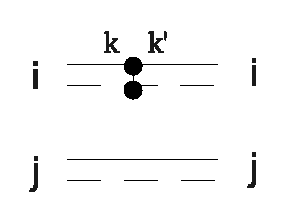
\includegraphics[width=0.2\textwidth]{image/tbdm2pair1.eps}\label{fig:tbdm2pair1}}\qquad
 \subfloat[][]{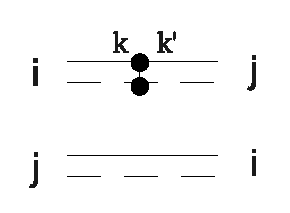
\includegraphics[width=0.2\textwidth]{image/tbdm2pair2.eps}\label{fig:tbdm2pair2}}\qquad
  \subfloat[][]{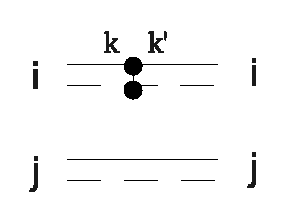
\includegraphics[width=0.2\textwidth]{image/tbdm2pair1.eps}\label{fig:tbdm2pair3}}\\
 \subfloat[][]{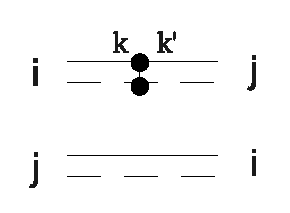
\includegraphics[width=0.2\textwidth]{image/tbdm2pair2.eps}\label{fig:tbdm2pair4}}\qquad
  \subfloat[][]{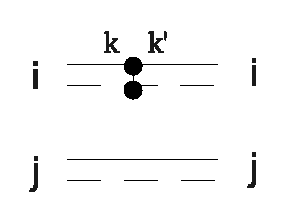
\includegraphics[width=0.2\textwidth]{image/tbdm2pair1.eps}\label{fig:tbdm2pair5}}\qquad
 \subfloat[][]{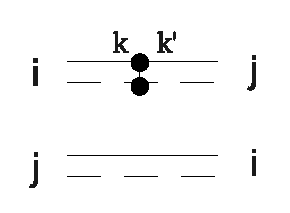
\includegraphics[width=0.2\textwidth]{image/tbdm2pair2.eps}\label{fig:tbdm2pair6}}\\
  \subfloat[][]{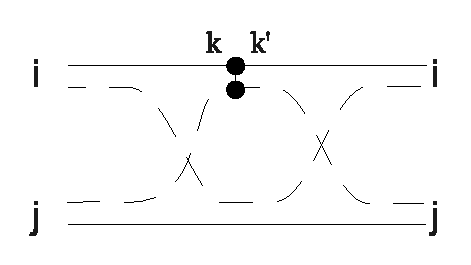
\includegraphics[width=0.3\textwidth]{image/tbdm2pair7.eps}\label{fig:tbdm2pair7}} 
\caption{Shiva diagram of two pairs }
\begin{description}
\item[\subref{fig:tbdm2pair1},\subref{fig:tbdm2pair2}] Signle pair without Pauli scattering.  There are also terms with $(i\leftrightarrow{j})$. First line of the above equation. 
\item[\subref{fig:tbdm2pair3},\subref{fig:tbdm2pair4},\subref{fig:tbdm2pair5},\subref{fig:tbdm2pair6}] Two-pair with Pauli scattering.  There are also terms with $(i\leftrightarrow{j})$. 
Second line of the equation. 
\item[\subref{fig:tbdm2pair7}] This coresponds the last term.  And there are the permutation of (i,j) as other terms.  
\end{description}
\end{figure}

The last term is especially interseting as this is two separate pieceses (fig.\ref{fig:shivaseparate}).  Normally, they do not exist, but here they do show up because we need pair of $\vk$,$\vk'$ .  
\begin{figure}[htb]\centering
 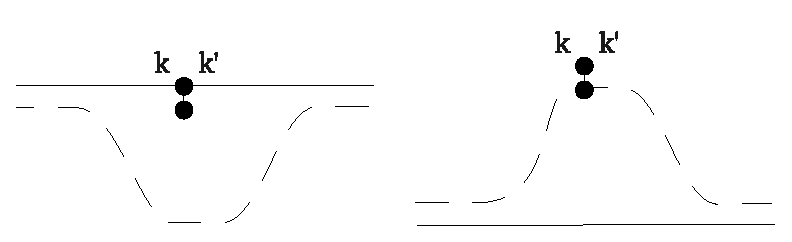
\includegraphics[width=0.3\textwidth]{image/shivaSeparate.eps}
\caption{Two separate connection parts of the last term of \eqref{eq:tbdm2pair}\label{fig:shivaseparate}}\centering
\end{figure}
And the normalization factor:
\begin{equation}
 {\avt{\Psi_2}{\Psi_2}}=\av{B^{}_j{}B^{}_i{}B^\dg_i{}B^\dg_j}=\avt{i}{i}\avt{j}{j}+\abs{\avt{i}{j}}^2-2\sum_\vk\avt{j}{\vk}\avt{i}{\vk}\avt{\vk}{i}\avt{\vk}{j}
\end{equation}

\subsubsection{Three pairs}
For a three-pair state $\ket{\Psi_3}=B^\dg_i{}B^\dg_j{}B^\dg_m\ket{\nu}$. 
we have 
\begin{equation}
\begin{split}
 \bra{\Psi_3}\beta^\dg_\vk=&\bra{\nu}B_m{}B_j{}B_i\beta^\dg_\vk\\
=&-2\avt{j}{\vk}\avt{m}{\vk}\bra{\nu}\beta_\vk{}B_i-2\avt{m}{\vk}\avt{i}{\vk}\bra{\nu}\beta_\vk{}B_j
-2\avt{i}{\vk}\avt{j}{\vk}\bra{\nu}\beta_\vk{}B_m\\
&+\avt{m}{\vk}\bra{\nu}B_i{}B_j+\avt{i}{\vk}\bra{\nu}B_j{}B_m+\avt{i}{\vk}\bra{\nu}B_m{}B_i\\
=&\br{-2\avt{i}{\vk}\avt{j}{\vk}\bra{\nu}\beta_\vk{}B_m+\avt{i}{\vk}\bra{\nu}B_j{}B_m}+(\mbox{i,j,m rotate permutation})
\end{split}
\end{equation}
We are lots of terms in the final expectation, like $\av{B^\dg{}B^\dg{}B^{}B^{}}$, $\av{\beta^\dg{}B^\dg{}B^{}B^{}}$,$\av{\beta^\dg{}B^\dg{}B^{}\beta^{}}$ , $\av{B^\dg{}B^\dg{}B^{}\beta^{}}$ .  
%\subsection{Variation method with the u,v,w}
We start with three hyperfine species a, b, c, where a is the common species in two channel. (a,b) is the open channel while (a,c) is the close channel. And the Hamiltonian is written in the form 
\begin{equation}
\begin{split}
 H=&\sum_\vk\epsilon^a_\vk{}a^+_\vk{}a^{}_\vk+\sum_\vk\epsilon^b_\vk{}b^+_\vk{}b^{}_\vk+\sum_\vk\epsilon^c_\vk{}c^+_\vk{}c^{}_\vk\\
  &+\nth{2}\sum_{\vk\vk'}U_{\vk\vk'}a^+_\vk{}b^+_{-\vk}{}b^{}_{-\vk'}a^{}_{\vk'}
	+\nth{2}\sum_{\vk\vk'}V_{\vk\vk'}a^+_\vk{}c^+_{-\vk}{}c^{}_{-\vk'}a^{}_{\vk'}\\
 &+\nth{2}\sum_{\vk\vk'}Y_{\vk\vk'}a^+_\vk{}b^+_{-\vk}{}c^{}_{-\vk'}a^{}_{\vk'}
	+\nth{2}\sum_{\vk\vk'}Y^*_{\vk\vk'}a^+_{\vk'}{}c^+_{-\vk'}{}b^{}_{-\vk}a^{}_{\vk}
\end{split} 
\end{equation}
By the Hermition condition we have 
\begin{equation}
 U_{\vk'\vk}=U^*_{\vk\vk'},\qquad{} V_{\vk'\vk}=V^*_{\vk\vk'}
\end{equation}
  We start from the ansatz as 
\begin{equation}\label{eq:ansatz}
 \ket{\Psi}=\prod_\vk\br{u_\vk+v_\vk{}a^\dg_\vk{}b^\dg_{-\vk}+w_\vk{}a^\dg_\vk{}c^\dg_{-\vk}}\ket{0}
\end{equation}
Here we require $\abs{u_\vk}^2+\abs{v_\vk}^2+\abs{w_\vk}^2=1$ for normalization.  For all the interaction term, there are two types of contribution,
for example, 
\begin{equation*}
\av{U_{\vk\vk'}a^\dg_\vk{}b^\dg_{-\vk}{}b^{}_{-\vk'}a^{}_{\vk'}}
=\sum_{\vk}U_{\vk\vk}\abs{v_\vk}^2+\sum_{\vk\neq\vk'}U_{\vk\vk'}v^{}_{\vk'}u^*_{\vk'}u^{}_\vk{}v^*_\vk
\end{equation*}
The first term is the Hatree term and the second term is more interesting pairing term.



And the free energy is 
\begin{equation}
 \begin{split}
  &F\equiv\av{H-\mu{}N}\\
    =&\sum(\xi^a_\vk+\xi^b_\vk)\abs{v_\vk}^2+\sum(\xi^a_\vk+\xi^c_\vk)\abs{w_\vk}^2\\
    &+\nth2\sum_{\vk}U_{\vk\vk}\abs{v_\vk}^2+\nth2\sum_{\vk\neq\vk'}U_{\vk\vk'}v^{}_{\vk'}u^*_{\vk'}u^{}_\vk{}v^*_\vk\\
    &+\nth2\sum_{\vk}V_{\vk\vk}\abs{w_\vk}^2
      +\nth2\sum_{\vk\neq\vk'}V_{\vk\vk'}w^{}_{\vk'}u^*_{\vk'}u^{}_\vk{}w^*_\vk\\
    &+\nth2\sum_{\vk}Y_{\vk\vk}w^{}_{\vk}v^*_\vk{}
      +\nth2\sum_{\vk\neq\vk'}Y_{\vk\vk'}w^{}_{\vk'}{u^{*}_{\vk'}}v^*_\vk{}u^{}_\vk\\
    &+\nth2\sum_{\vk}Y^*_{\vk\vk}w^*_{\vk}v^{}_{\vk}{}
      +\nth2\sum_{\vk\neq\vk'}Y^*_{\vk\vk'}w^*_{\vk}{u^{}_{\vk}}v^{}_{\vk'}{}u^{*}_{\vk'}
 \end{split}
\end{equation}
Where 
\begin{equation*}
 \xi^a_\vk=\epsilon^a_\vk-\mu^a,\qquad\xi^b_\vk=\epsilon^b_\vk-\mu^b,\qquad\xi^c_\vk=\epsilon^c_\vk-\mu^b
\end{equation*}
The chemical potential is added to make sure the $n_a=n_b+n_c=\nth{2}n$.
 I drop the Hatree term as this in some sense just shift the chemical potentials as it only relates to the density.  (\emph{Not sure still valid in the two-channel problems, especially for the close-channel.})  Also, I ignore the summation on the second only goes through $\vk\neq\vk'$ as the correction is in the higher order. 
 
Now introduce the parameters $\theta_\vk$, $\phi_\vk$ to include the normalization condition.  
\begin{equation}
 u_{\vk}=\cos\theta_\vk,\qquad{} v_{\vk}=\sin\theta_\vk\cos\phi_\vk,\qquad{}
 w_{\vk}=\sin\theta_\vk\sin\phi_\vk
\end{equation}
We take them as real quantities as those that minimize the free energy are real.(?) Now the free energy can be written as 

\begin{equation}
 \begin{split}
  F=&\sum\xi^{ab}_\vk\sin^2{\theta_\vk}\cos^2\phi_\vk+\sum\xi^{ac}_\vk\sin^2{\theta_\vk}\sin^2\phi_vk\\
    &+\nth2\sum_{\vk\vk'}U_{\vk\vk'}\cos\theta_{\vk'}\sin\theta_{\vk'}\cos\phi_{\vk'}\cos\theta_\vk{}\sin\theta_\vk\cos\phi_\vk\\
    &+\nth2\sum_{\vk\vk'}V_{\vk\vk'}\cos\theta_{\vk'}\sin\theta_{\vk'}\sin\phi_{\vk'}\cos\theta_\vk{}\sin\theta_\vk\sin\phi_\vk\\
    &+\nth2\sum_{\vk\vk'}Y_{\vk\vk'}\cos\theta_{\vk'}\sin\theta_{\vk'}\cos\phi_{\vk'}\cos\theta_\vk{}\sin\theta_\vk\sin\phi_\vk\\
    &+\nth2\sum_{\vk\vk'}Y^*_{\vk\vk'}\cos\theta_{\vk'}\sin\theta_{\vk'}\sin\phi_{\vk'}\cos\theta_\vk{}\sin\theta_\vk\cos\phi_\vk\\
    =&\nth4\sum_\vk\xi^{ab}_\vk(1-\cos2\theta_\vk)(1+\cos2\phi_\vk)+\nth4\sum_\vk\xi^{ac}_\vk(1-\cos2\theta_\vk)(1-\cos2\phi_\vk)\\
    &+\nth{8}\sum_{\vk\vk'}U\sin2\theta_\vk\cos\phi_\vk\sin2\theta_{\vk'}\cos\phi_{\vk'}+\nth{8}\sum_{\vk\vk'}V\sin2\theta_\vk\sin\phi_\vk\sin2\theta_{\vk'}\sin\phi_{\vk'}    \\
    &+\nth{4}\sum_{\vk\vk'}Y\sin2\theta_\vk\cos\phi_\vk\sin2\theta_{\vk'}\sin\phi_{\vk'}    
 \end{split}
\end{equation}
We assume that $Y=Y^*$. From the above equation, we can differentiate it with respect to $\theta_\vk$ and $\phi_\vk$ and set the derivative as 0, therefore minimize free energy. 
\begin{align}
0=&\pdiff{F}{\theta_\vk}\notag\\
 =&\nth{2}\sin2\theta_\vk\mbr{\xi^{ab}_\vk(1+\cos2\phi_\vk)+\xi^{ac}_\vk(1-\cos2\phi_\vk)}\notag\\
 &+\nth2\sum_{\vk'}\cos2\theta_\vk\sin2\theta_{\vk'}\mbr{U\cos\phi_\vk\cos\phi_{\vk'}+V\sin\phi_\vk\sin\phi_{\vk'}+Y\sin(\phi_{\vk'}+\phi_\vk)}\\
 0=&\pdiff{F}{\phi_\vk}\notag\\
 =&-\nth{2}(\xi^{ab}_\vk-\xi^{ac}_\vk)\sin2\phi_\vk(1-\cos2\theta_\vk)\notag\\
 &-\nth4\sum_{\vk'}\sin2\theta_\vk\sin2\theta_{\vk'}\mbr{U\sin\phi_\vk\cos\phi_{\vk'}-V\cos\phi_\vk\sin\phi_{\vk'}-Y\cos(\phi_{\vk'}+\phi_\vk)}
\end{align}
  These two set of equations (for each $\vk$, but decoupled) fully determine the wave-function. 
We introduce two quantities:
\begin{align}
\Delta_\vk^U&=\sum_{\vk'}\sin2\theta_{\vk'}(U_{\vk\vk'}\cos\phi_{\vk'}+Y_{\vk\vk'}\sin\phi_{\vk'})\label{eq:gap1}\\
\Delta_\vk^V&=\sum_{\vk'}\sin2\theta_{\vk'}(V_{\vk\vk'}\sin\phi_{\vk'}+Y_{\vk\vk'}\cos\phi_{\vk'})\label{eq:gap2}
\end{align} 
As we can see eqs.(\ref{eq:gap1},\ref{eq:gap2}) is indeed very similar to the structure of two-body Schr\"{o}‌dinger equation.
If we ‌introduce the Zeeman energy detuning between two channels
\begin{equation}
\eta=\xi^{ab}-\xi^{ac}
\end{equation}
These equations can be written into a more compact form
\begin{align}
\tan2\theta_\vk&=-\frac{\cos\phi_\vk\Delta^U_\vk+\sin\phi_\vk\Delta^V_\vk}{2\xi^{ab}_\vk+2\eta\cos^2\phi_\vk}\label{eq:tan1}\\
\tan\theta_\vk&=-\frac{\sin\phi_\vk\Delta^U_\vk-\cos\phi_\vk\Delta^V_\vk}{2\eta\sin2\phi_\vk}\label{eq:tan2}
\end{align} 


Furthermore, when $k\rightarrow\infty$, from eq. (\ref{eq:tan1}), we see that $\theta\rightarrow0$ as $1/\xi$;  and from eq. (\ref{eq:tan2}), we see that $\sin\phi_\vk\Delta^U=\cos\phi_\vk\Delta^V$ as we assume $\Delta$ varies slowly over $\vk$.  We have 
\begin{align*}
\cos^2\phi_\vk&=\frac{{\Delta^U}^2}{{\Delta^V}^2+{\Delta^U}^2}\\
\sin^2\phi_\vk&=\frac{{\Delta^V}^2}{{\Delta^V}^2+{\Delta^U}^2}
\end{align*}
And 
\[\tan2\theta_\vk=-\frac{({{\Delta^V}^2+{\Delta^U}^2})^{1/2}}{2\xi^{ab}_\vk}\]

Eqs. (\ref{eq:gap1},\ref{eq:gap2}) are similar as those derived from the Green's function method in the eq. (\ref{eq:gapMatrix}), and should be able to renormalized in the similar fashion $\Delta=T(F-G\Delta)$, where in our notation $({F^o,F^c})=(\cos\theta_\vk\sin\theta_\vk\cos\phi_\vk,\cos\theta_\vk\sin\theta_\vk\sin\phi_\vk)$.  The problem, however, is that the eqs. (\ref{eq:tan1},\ref{eq:tan2}) does not present a simple analytic solution about $\theta$ and $\phi$ in terms of $\Delta$ and therefore the gap equations cannot be written into a simple renormalized  equation although they are implicit functions of $\Delta$.
 It is a rather cumbersome process to calculate the integration in renormalized gap equations.  Furthermore, information of the close-channel is close to a simple one-level bound-state is not fully incorporated and the equation might be simpler and has a nicer form if I can manage to do that.  

\subsection{more thoughts}
From eqs. (\ref{eq:gap1},\ref{eq:gap2}), $\Delta^{U,V}_\vk$ varies slowly with $k$ if interaction depends on momentum weakly, at least for low momentum.  Therefore, in the renomalization, they can be taken as constants.  In that case, eqs. (\ref{eq:tan1},\ref{eq:tan2}) determine $\theta_k(\xi_k,\Delta^U,\Delta^V)$ and $\phi_k(\xi_k,\Delta^U,\Delta^V)$, which in turn give two-body wave-function $F^{o,c}_k(\xi_k,\Delta^U,\Delta^V)$.  
With the renomalized gap equation,.  
\begin{equation}\label{eq:renomal1}
\begin{pmatrix}\Delta^U\\\Delta^V\end{pmatrix}=\begin{pmatrix}T_{oo}&T_{oc}\\T_{co}&T_{cc}\end{pmatrix}
\begin{pmatrix}\sum{F^o-\frac{\Delta^U}{2\epsilon}}\\\sum{F^c-\frac{\Delta^V}{2\epsilon+\eta}}\end{pmatrix}
\end{equation}
and the number equation, should give us three parameters in the problems: $\Delta^{U,V}$ and $\mu$.  The close-channel infomation is incorporated into the $T$-matrix.  The problem is more about the computation difficulty as there is no simple analytic solution for $F^{o,c}$, therefore, eq. (\ref{eq:renomal1}) cannot be done easily.

What happened in the broad-resonance limit? Or very BEC/BCS end? 

\subsection{T-matrix}
Follow \cite{JacksonNarrow}, the bare interaction $V$ should have the form \footnote{notice the some change of notation}
\begin{equation}
V(r)=\frac{V_s(r)+3V_t(r)}{4}+\mbr{V_t(r)-V_s(r)}\mathbf{S_1}\cdot\mathbf{S_2}
\end{equation}
we can establish the T-matrix from $V$.
\begin{equation}
 {\fmtrx{T_{cc}}{T_{co}}{T_{oc}}{T_{oo}}}^{-1}={\fmtrx{V_{cc}}{V_{co}}{V_{oc}}{V_{oo}}}^{-1}-{\fmtrx{G_{c}}{0}{0}{G_{o}}}
\end{equation}
For 0-temperature, pair propagators $G_o$ and $G_c$ are
\begin{equation}
 G_o(\omega,\vK,\vq)=\nth{\omega+i\delta-\frac{K^2}{4m}-\frac{q^2}{m}}
\end{equation}
\begin{equation}
 G_c(\omega,\vK,\vq,B)=\nth{\omega+i\delta-\eta(B)-\frac{K^2}{4m}-\frac{q^2}{m}}
\end{equation}
where $E_{th}(B)$ is the detuning, depending on magnatic field $B$. Here we can break it down into two steps. First, introduce 
 \begin{equation}
 {\fmtrx{U_{cc}}{U_{co}}{U_{oc}}{U_{oo}}}^{-1}={\fmtrx{V_{cc}}{V_{co}}{V_{oc}}{V_{oo}}}^{-1}-{\fmtrx{G^{vac}}{0}{0}{G^{vac}}}
\end{equation}
where $G^{vac}(q)=(i\delta-q^2/m)^{-1}$ is the vacuum pair propagator ignoring the hyperfine splitting at $\omega=0$ and no center momentum $\vK$.  Furthermore, when the close-channel resonnant state is close to threshold and well-seperated from other discrete levels, the effective interaction is separable.  So 
\begin{equation}
 U(\vq',\vq)=\frac{4\pi}{m}\mbr{\frac{a_s+3a_t}{4}+(a_t-a_s)\mathbf{S_1}\cdot\mathbf{S_2}}g(q')g(q)
\end{equation}
$g(q)\rightarrow0$ for $qr_C\rightarrow\infty$ where $r_C$ is the interaction range.  But This can be projected to the hyperfine-spin space and therefore two-channel.  
\begin{equation}
 {\fmtrx{U_{cc}}{U_{co}}{U_{oc}}{U_{oo}}}=
\frac{4\pi}{m}\mbr{\fmtrx{\frac{c_7a_s+a_t}{1+c_7}}{\frac{a_t-a_s}{\sqrt{1+c_7}\sqrt{1+c_9}}}
{\frac{a_t-a_s}{\sqrt{1+c_7}\sqrt{1+c_9}}}{\frac{c_9a_s+a_t}{1+c_9}}}
\end{equation}
For example, $\ket{9/2,-9/2}$, $\ket{9/2,-7/2}$, $\ket{7/2,-7/2}$ of ${}^{40}K$ at resonance $B=201.6$, $c_7=14.9$ and $c_9=0.059$ Note that both $c_7$ and $c_9$ depends on B.  

The second step deals with the influence of $B$ in the theshold $E_{th}$ as well as the energy dependence of $G$. 
 \begin{equation}
  {\fmtrx{T_{cc}}{T_{co}}{T_{oc}}{T_{oo}}}^{-1}={\fmtrx{U_{cc}}{U_{co}}{U_{oc}}{U_{oo}}}^{-1}-{\fmtrx{\Delta{}G_c}{0}{0}{\Delta{}G_o}}
\end{equation}
where $\Delta{}G_{o/c}=G_{o,c}(\omega,\vK,\vq,B)-G^{vac}(q)$.  Using the seperable properties of $U$, we can concentrate the $\vq$ dependence on two quantities and this leaves us a simple two-by-two algebra matrix equation.  
\begin{equation}
\Pi_{o,c}(\omega,\vK,B)=\int\frac{d^3q}{(2\pi)^3}\Delta{}G_{o,c}g^2(q)                  
\end{equation}
where for the contact interaction with $r_C=0$, we find $\Pi_o(\omega,\vK)=-im^{3/2}\sqrt{\omega-K^2/(4m)}$ and $\Pi_c(\omega,\vK,B)=\Pi_o(\omega-E_{th}(B),\vK)$
Especially, for $\omega=0$ and no central mometum $\vK$, $\Pi_o=0$ and $\Pi_c=\sqrt{-\eta(B)}$
\begin{gather}\label{eq:T}
 T_{cc}=\frac{U_{cc}}{1-U_{cc}\Pi_c}\\
T_{oc}=T_{co}=\frac{U_{oc}}{1-U_{cc}\Pi_c}\\
T_{oo}=U_{oo}+\frac{U_{oc}^2\Pi_c}{1-U_{cc}\Pi_c}
\end{gather}
comparing this with the commonly used formula 
\begin{equation}
 T_{oo}=\frac{4\pi{}a_{bg}}{m}\br{1-\frac{\Delta{}B}{B-B_0}}
\end{equation}
We find the resonance position $B_0$ satisfies
\begin{equation}
 1-U_{cc}(B_0)\Pi_c(B_0)=0
\end{equation}
And other quantities, such as $a_s$, $a_t$ can be expressed with the experimental quantities. 

However, it is still not clear to me how to really map broad /narrow resonance into the many-body eq.(\ref{eq:renomal1}) in a calculable sense.  The criteria of broad resonance as in \cite{JacksonNarrow} is   
\begin{equation}\label{eq:broadCriteria}
\Delta\mu\Delta{}B\gg\frac{k_F}{ma_{bg}}
\end{equation}


\subsection{rescale with Fermi momemtum/energy}
If we rescale renormalized gap equation eq. \ref{eq:renomal1} and the number equation with the Fermi momentum/energy, we have 
\begin{equation}\label{eq:renormal2}
\begin{pmatrix}\widetilde\Delta^U\\\widetilde\Delta^V\end{pmatrix}=
8\pi{a}{k_F}\begin{pmatrix}1&T_{oc}/T_{oo}\\T_{co}/T_{oo}&T_{cc}/T_{oo}\end{pmatrix}
\int\widetilde{k}^2d\widetilde{k}
\begin{pmatrix}
\nth{2}\sin2\theta_{k}\cos\phi_k-\frac{\widetilde\Delta^U}{2\widetilde\epsilon}\\
\nth{2}\sin2\theta_{k}\sin\phi_k-\frac{\widetilde\Delta^U}{2\widetilde\epsilon+\widetilde{\eta}}
\end{pmatrix}
\end{equation}
and rescaled number equation
\begin{equation}
 \int\widetilde{k}^2\sin^2\theta_kd\widetilde{k}=\nth{3}
\end{equation}
We can find the criteria of broad resonance (eq. \ref{eq:broadCriteria}) becomes 
\begin{equation}
 ak_F\widetilde{\eta}\gg1 
\end{equation}
Here we use $a=a_{bg}(1+\Delta_B/(B-B_0)$,  ignoring constant $1$ around the resonance, and also use the fact that rougly $\eta=\Delta\mu(B-B_0)$. At the broad limit, term $\frac{\widetilde\Delta^U}{2\widetilde\epsilon+\widetilde{\eta}}$ of the second integration in eq. \ref{eq:renormal2} gives a negligible contribution when $\sin2\theta_k$ is substantial.  So a simple solution is to put $\cos\phi_k\approx1$ while $\sin\phi_k\approx0$ for where $\sin2\theta_k$ is substantial (i.e. the particle is concentrated in open-channel).  Therefore, we reduce the two-channel problems into one-channel problem, omitting the close-channel. Here, we can see the interplaying between fermi energy and the two-body quantities, whether eq. \ref{eq:renormal2} can be reduced to a single-channel problem is due to the size of $\widetilde{\eta}$, which is determined by the ratio of the deturning and Fermi energy.  
%\section{note of 2009.12.07}
%\subsection{Spherical harmonic and Fourier transformation}
From (34.3) of \cite{landau}, we have
\begin{equation}
e^{i\vk\cdot\vr}=4\pi\sum_{l=0}^{\infty}\sum_{m=-l}^{l}i^l{}j_l(kr)Y^*_{lm}(\hat{k})Y_{lm}(\hat{r})
\end{equation}
We find the the Fourier tansformation in 3D of the spherical harmonic function does not change $(lm)$,
\begin{equation}
\int{d\hat{k}e^{i\vk\cdot\vr}Y_{lm}(\hat{k})}=4\pi{}i^l{}j_l(kr)Y_{lm}(\hat{r})
\end{equation} 
And 
\begin{equation*}
\Psi(\vr)=\sum_{l=0}^{\infty}\sum_{m=-l}^{l}\int{dk}\psi_{lm}{(k)}\int{d\hat{k}e^{i\vk\cdot\vr}Y_{lm}(\hat{k})}=4\pi{}\sum_{l=0}^{\infty}\sum_{m=-l}^{l}i^l{}Y_{lm}(\hat{r})\int{dk}\psi_{lm}{(k)}j_l(kr)
\end{equation*}
So the $(lm)$ component of real-space relates only to the $(lm)$ component of k-space 
\begin{equation}
\psi_{lm}(r)=4\pi{}i^l{}\int{dk}\psi_{lm}{(k)}j_l(kr)
\end{equation}


\subsection{Shizhong's comment\label{subsec:20091207}}
He think besides open-channel affects close-channel in statistics, there is also the statistical effect from close-channel to open-channel.  And finally, one can include both coherently. Numerically, one can do these two things iterately and maybe find the many-body result. There are also kinetical interaction and the full treatment involve the $2\times2$.   

\textit{My thinking:The assumption that close-channel molecule is large and close-to-threshhold, actually increases the statistical effect of close-channel to open-channel because close-channel is then denser in k-space.  	}

He has doubts to characterize the close-channel bound-state with one single parameter $a_s$, but he agrees that this might be OK for a model.  I think it is fine given the condition that close-channel is close-to-threshold and very large.  

\subsection{}
Some arguments in last section \ref{sec:20100908:idea} seems incorrect, at least the argument that in close-channel zero-blocked  or one-pair-blocked within $k_{c}$ dominated multi-pair-blocked situation for open-channel BCS ansatz seems incorrect.  Therefore the argument in the following section \ref{sec:20100908:cal} becomes more or less irrelevant.  Nevertheless, the observation that close-channel bound state is relatively small in real space and therefore much extended in k-space is still useful.  Looked back \eef{eq:uvw:F}, (ignored Hatree terms)
\begin{equation}\tag{\ref{eq:uvw:F}}
 \begin{split}
  &F\equiv\av{H-\mu{}N}\\
    =&\sum(\xi^{ab}_\vk)\abs{v_\vk}^2+\nth2\sum_{\vk\neq\vk'}U_{\vk\vk'}v^{}_{\vk'}u^*_{\vk'}u^{}_\vk{}v^*_\vk\\
    &+\sum(\xi^{ac}_\vk)\abs{w_\vk}^2
      +\nth2\sum_{\vk\neq\vk'}V_{\vk\vk'}w^{}_{\vk'}u^*_{\vk'}u^{}_\vk{}w^*_\vk\\
    &  +\nth2\sum_{\vk\neq\vk'}Y_{\vk\vk'}w^{}_{\vk'}{u^{*}_{\vk'}}v^*_\vk{}u^{}_\vk
        +\nth2\sum_{\vk\neq\vk'}Y^*_{\vk\vk'}w^*_{\vk}{u^{}_{\vk}}v^{}_{\vk'}{}u^{*}_{\vk'}
 \end{split}
\end{equation}
It is useful to recognize that $w_{\vk}$ (or maybe $G_{\vk}=u_{\vk}w_{\vk}$) is always small. Changing  $w_{\vk}$ into $G_{\vk}$ in term $\sum(\xi^{ac}_\vk)\abs{w_\vk}^2$ introduces two problems:  First, the $w_{\vk}$ is finite, but it is small and error is probably small too;  second, within $k_{c}$, $v_{\vk}$ is substantial and therefore reduce the $u_{\vk}$ and makes $G_{\vk}$ much smaller than $w_{\vk}$, the error introduced here is probably also small because $w_{\vk}$ is small within $k_{c}$ and therefore the summation is small comparing to the term itself.  
So we have the free energy as 
\begin{equation}\label{eq:20100909:F}
 \begin{split}
    F=&\sum(\xi^{ab}_\vk)\abs{v_\vk}^2+\nth2\sum_{\vk\neq\vk'}U_{\vk\vk'}F^{}_{\vk'}F^*_\vk\\
    &+\sum(\xi^{ac}_\vk)\abs{G_\vk}^2
      +\nth2\sum_{\vk\neq\vk'}V_{\vk\vk'}G^{}_{\vk'}G^*_\vk\\
    &  +\nth2\sum_{\vk\neq\vk'}Y_{\vk\vk'}G^{}_{\vk'}F^*_\vk{}
        +\nth2\sum_{\vk\neq\vk'}Y^*_{\vk\vk'}G^*_{\vk}F^{}_{\vk'}
 \end{split}
\end{equation}
Take $F_{\vk}$ and $G_{\vk}$ as variables, first we express $v_{\vk}$ in term of them.  We have  $\abs{u_\vk}^2+\abs{v_\vk}^2+\abs{w_\vk}^2=1$, here we replace  $w_{\vk}$  with  $G_{\vk}$  again.  We have 
\[
\begin{split}
v_{\vk}^2=&\nth{2}(1-G_{\vk}^{2}+\sqrt{(1-G_{\vk}^{2})^{2}-4F_{\vk}^{2}})\qquad (\epsilon_{\vk}<\mu)\\
	=&\nth{2}(1-G_{\vk}^{2}-\sqrt{(1-G_{\vk}^{2})^{2}-4F_{\vk}^{2}})\qquad (\epsilon_{\vk}\geq\mu)
\end{split}
\]
In BEC side ($\mu<0$), only the second form exists. (This sign problem is not important anyway as we can freely add a overall phase to $F_{\vk}$ or $u,v$, as mostly we just deal with the square of these quantities. ).   Just put the second case into the free energy \eef{eq:20100909:F}, take derivative over $F_{\vk}$, (take it as real, not complex) we find 
\begin{equation}\label{eq:20100909:fEq}
\epsilon^{ab}_{\vk}(\frac{2F_{\vk}}{\sqrt{(1-G_{\vk}^{2})^{2}-4F_{\vk}^{2}}})+\sum_{\vk'}(U_{\vk\vk'}F_{\vk'}+Y_{\vk\vk'}G_{\vk'})=0
\end{equation}
Define the normal gap parameters 
\begin{equation}\label{eq:20100909:gap}
\Delta^{F}_{\vk}=-\sum_{\vk'}(U_{\vk\vk'}F_{\vk'}+Y_{\vk\vk'}G_{\vk'})
\end{equation}
And we find
\begin{equation}
F_{\vk}=\frac{(1-G_{\vk}^{2})\Delta^{F}_{\vk}}{2\sqrt{(\epsilon^{ab}_{\vk}-\mu)^{2}+\Delta^{F}_{\vk}{}^{2}}}
\end{equation}
For low-k ($k<k_{c}$), both $U_{\vk\vk'}$ and $Y_{\vk\vk'}$ varies slowly, so $\Delta^{F}_{\vk}$ varies slowly and we can drop subscript $\vk$ and treat it as constant.  \eef{eq:20100909:fEq} describe the many-body effects when comparing with the two-body Schr\"{o}dinger equation.  $(1-G^{2})$ gives the pauli exclusion from the close-channel, the square root takes into account the pauli exclusion within open-channel.  

\eef{eq:20100909:gap} cannot be renormalized due to the extra factor $(1-G_{\vk}^{2})$.  A close look reveal that it does not reduce to normal \sch equation due to this extra factor.  This is puzzling.  It might be caused by replace $w_{\vk}$ with $G_{\vk}$.  Another possibility is that the coupled equation cannot be renormalized in this way, it has to be renormalized in the two-channel fashion, for the diagonalized  basis.  

\subsection{Tony's comment}
Tony takes \eef{eq:20100909:gap} as renormalized density of states.  From there, the two-body problem is also modified for this renormalized DoS. 

He suggested me to take $u_{\vk}$ as single-channel result for $G_{\vk}$.   

He encourage me to think about whether close-channel is significantly modified within $k_{F}$, he does not give me a definitive answer.  I feel this might relate to the real close-channel potential that support the bound state.  Not clear idea anyway.  
------ This is probably not modified as close-channel is much higher due to Zeeman energy.  This bare detuning corresponding the size of the close-channel bound state and therefore larger than any other energy scale.   It is the bound state level that close to 0 of open-channel.  By simple energy consideration, it is very disadvantageous to populate any close-channel low k state at all due to the high kinetic energy (with Zeeman energy).  It is only energetic feasible to populate it in the bound-state way where the potential energy gaining is sufficient to compensate the large kinetic energy.  

He also stress that I need to keep an eye on things thrown away in approximation,  whether they are in the order of kept terms.  

\subsection{}
The difference between $w_{\vk}$ and $G_{\vk}$ are introduced because of the grand-canonical nature of the ansatz?  In BCS side, this introduce really small error as $\Delta{N}$ can be shown are small.  Does that hold in BEC end?
\begin{equation}
\Delta{N}=\av{N-N^{2}}=\sum{\abs{v_{\vk}}^{2}-\abs{v_{\vk}}^{4}}=\sum{\abs{F_{\vk}}^{2}}
	=\sum{\abs{\frac{\Delta}{2E}}^{2}}
\end{equation}
This is extremely small for the BCS-side, but not the case in BEC-end.  (\emph{Interesting problem!})

One thing potentially useful is that to distinguish the region within $k_{c}$ and without where $G_{\vk}$ ($w_{\vk}$) is small comparing to open-channel or not.  
\subsection{Single channel problem}
From \eef{eq:20100909:fullgap}, the single-channel equation is 
\begin{equation}
\frac{2F_{\vk}}{\sqrt{1-4 F_{\vk}^2}} \epsilon^{ab}_{\vk}+U_{\vk\vk'}F_{\vk'}=0
\end{equation}
The factor $\nth{\sqrt{1-4 F_{\vk}^2}}$ gives the many-body correction comparing to two-body \sch equation.  This factor is significant when $F_{\vk}$ is large.  In BCS, this is near Fermi surface;  in BEC, all $F_{\vk}$ is small, and therefore, the equation is closer to \sch  equation.  This is understandable because that there are much less overlapping for BEC, where molecule (overlapping) is small.  

In each equation of \eef{eq:20100909:fullgap},  the first term clearly involves the pauli exclusion of the channel itself as well as from the other channel;  the second terms seems to be in higher order due to statistics;  the third term is the normal inner-channel interaction; and the last term is the inter-channel interaction.  In the first term of the second equation,  $F_{\vk}$ should be larger than $G_{\vk}$ in low-k ($k_{F}$)and indicates that the inter-channel exclusion is more important than inner-channel effect.  This makes sense as open channel weight is larger in low k.  

\subsection{}
A term as $Y_{\vk\vk'}F_{\vk'}$ is fine in BEC side, but in BCS side, $F_{\vk}$ significantly differs from $v_{\vk}$ in low k and this terms seems significantly smaller than the case in two-body. 

In the first equation of \eef{eq:20100909:fullgap}, inter-channel interaction $Y_{\vk\vk'}G_{\vk'}$ gets large in resonance because it pulls the components also from high k of $G_{\vk'}$, while the pauli exclusion only comes from the single $G_{\vk}$, which seems always small.  

Key seems still in the two-body problem in this exact same representation and then we can renormalize it.  This serves two purpose: renormalize the high-k divergence and provide the comparison of two-body quantity $a_{s}$.

\subsection{}
It is energetically very disadvantageous to diviate from the resonant bound state, furthermore, it is very small in k-space as the bound-state is relatively small.  Therefore, as the first order approximation, we drop the second term and the denominator in the first term of the second equation (close-channel) of \eef{eq:20100909:fullgap}\footnote{ This is certainly OK for he BEC end where $F_{k}\ll1$ all the time.  It is more subtle when $F_{k}$ is close to maximum $\nth2$, this happens around Fermi energy in BCS limit, but the approximation is still OK for other places. So at least for bulk of the region of $G_{\vk}$ satisfies \eef{eq:20100915:gapb}}.  In the first equation, we drop the factor $\left(1+\sqrt{1-4 F_{\vk}^2-4 G_{\vk}^2}\right)^2$ in the second term for easier calculation, (no strong reason yet), the second term is relatively minor comparing to the first. We write down the approximated equations
\begin{subequations}\label{eq:20100915:gap}
\begin{gather}\label{eq:20100915:gapa}
\frac{2F_{\vk}}{\sqrt{1-4 F_{\vk}^2-4 G_{\vk}^2}} (\epsilon^{ab}_{\vk}+  G_{\vk}^2\eta)+U_{\vk\vk'}F_{\vk'}+Y_{\vk\vk'}G_{\vk'}=0\\
\label{eq:20100915:gapb}
{2G_{\vk}}(\epsilon^{ab}_{\vk}+\eta)+V_{\vk\vk'}G_{\vk'}+Y_{\vk\vk'}F_{\vk'}=0
\end{gather}
\end{subequations}
If $G_{\vk}=\alpha\phi^{0}_{\vk}$ as $\phi_{\vk}^{0}$ is the solution for the isolated close-channel \sch.  
\[
{2\phi^{0}_{\vk}}(\epsilon_{\vk})+V_{\vk\vk'}\phi^{0}_{\vk'}=-E^{0}\phi^{0}_{\vk'}
\]
\eef{eq:20100915:gapb} becomes
\begin{equation}
G_{\vk}=\frac{Y_{\vk\vk'}F_{\vk'}}{2(E^{0}-\eta)}
\end{equation}
Plug this back into the last term of \eef{eq:20100915:gapa}, we have 
\begin{equation}
\frac{2F_{\vk}}{\sqrt{1-4 F_{\vk}^2-4 G_{\vk}^2}} (\epsilon^{ab}_{\vk}+  G_{\vk}^2\eta)+U_{\vk\vk'}F_{\vk'}+\frac{Y_{\vk\vk'}Y_{\vk'\vk''}}{2(E^{0}-\eta)}F_{\vk''}=0
\end{equation}
Now considering the last two terms has weak dependecy in low k, we can set 
\begin{equation}\label{eq:20100915:gap1}
\frac{2F_{\vk}}{\sqrt{1-4 F_{\vk}^2-4 G_{\vk}^2}} (\epsilon^{ab}_{\vk}+  G_{\vk}^2\eta)\equiv\Delta_{\vk}=-(U_{\vk\vk'}F_{\vk'}+\frac{Y_{\vk\vk'}Y_{\vk'\vk''}}{2(E^{0}-\eta)}F_{\vk''})
\end{equation}
We can express $F_{\vk}$ according to $\Delta_{\vk}$,  (ignore the higher order of $G_{\vk}$)
\begin{equation}
F_{\vk}=\frac{\Delta_{\vk}}2\sqrt{\frac{(1-4G_{\vk}^{2})}{(\epsilon_{\vk}^{2}+\Delta_{\vk}^{2}+2G_{\vk}^{2}\eta\epsilon_{\vk})}}
\end{equation}
Put it back into the second half of gap equation (\ref{eq:20100915:gap1}), 
\[
\Delta_{\vk}=-\sum_{\vk'}\br{U_{\vk\vk'}+\frac{Y_{\vk\vk''}Y_{\vk''\vk'}}{2(E^{0}-\eta)}}\frac{\Delta_{\vk'}}2\sqrt{\frac{(1-4G_{\vk'}^{2})}{(\epsilon_{\vk'}^{2}+\Delta_{\vk'}^{2}+2G_{\vk'}^{2}\eta\epsilon_{\vk'})}}
\]
At low k, $\Delta_{\vk}$ has weak dependency on k and we can take $\Delta_{\vk'}$ out of the summation,  then go through the same procedure as in \cite{Leggett,Fetter} to renormalize the equation
\begin{equation}\label{eq:20100915:renormGap}
\nth{\tilde{t_{0}}}=-\sum_{\vk'}\sqrt{(1-4G_{\vk'}^{2})}
\br{\nth{\epsilon_{\vk'}}-\nth{\sqrt{(\epsilon_{\vk'}^{2}+\Delta^{2}+2G_{\vk'}^{2}\eta\epsilon_{\vk'})}}}
\end{equation}
Noted that $t_{0}$ is the zero-energy scattering amplitude for a reduced density of energy by factor $\sqrt{(1-4G_{\vk'}^{2})}$.  
\begin{gather}
\tilde{t_{0}}=\br{1-\tilde{U}\tilde{ K}}^{-1}\tilde{U}\label{eq:20100915:t0}\\
\tilde{U}_{\vk\vk'}=\nth{2} \br{U_{\vk\vk'}+\frac{Y_{\vk\vk''}Y_{\vk''\vk'}}{2(E^{0}-\eta)}}\label{eq:20100915:tu}\\
\tilde{K}=\frac{\sqrt{1-4G_{\vk}^{2}}}{\epsilon_{\vk}}\delta_{\vk\vk'}
\end{gather}
This is a little odd as the two-body quantity $t_{0}$ is affected by the many-body quantity $G_{\vk}$.  Nevertheless, it seems OK to simply use the two-body close-channel bound-state wave function as $G_{\vk}$ for the lowest order approximation.   Of course, in higher order, especially, the BCS case, the open-channel is significantly different from the two-body solution and therefore the weight is significantly different, from \eef{eq:20100915:gapb}, this affect the weight of close-channel $G_{\vk}$.  Unlike the many-body equation \eef{eq:20100915:renormGap}, where only low-k is interesting and therefore $G_{\vk}$ can be regarded as constant and small, the summation should go all the way to high-k.  As \eef{eq:20100915:tu}, $\tilde{U}$ is the unmodified, the resonance position is probably not modified, but the width of resonance is changed.  



\subsection{Tony's comment}
Tony suggested that in \eef{eq:20100915:renormGap} we only need to care about the $G_{\vk'}$ where the difference in summation is substantial.  

He mentioned that in normal BEC, below $T_{C}$ the fluctuation of paritcle is very large for gand cannonical emsemble.  That might have to do with the problem in Sec \ref{sec:20100915:deltaN}.
\subsection{Two effects of narrow resonance}
There are two possibilities for narrow resonance:  
\begin{enumerate}
\item Pauli exclusion for three species, where the close-channel weight is large.  
\item Fermi energy is larger than the width that scattering amplitude (NOT $a_{s}$) changes the sign.  Therefore $a_{s}$ is no longer a good indicator for the interaction.  However, it might still be OK to take $a_{s}$ simply as the quantity introduced by renormalization.   This has been explored by several papers already \cite{NarrowJensen1,NarrowJensen,GurarieNarrow}.  
\end{enumerate}
Four species case can fall into narrow resonance in  the second sense.  \cite{NarrowJensen1,NarrowJensen} uses the single-channel approach but a T-matrix with effective range $r_{0}$, the narrow resonance is $r_{0}k_{F}\ll1$.  In \cite{NarrowJensen}, a single-channel bare interaction is assumed and (unnormalized) gap, number equations  are  solved numerically with different interaction parameters corresponding to different effective ranges. The result is some small corrections in gap, chemical potential...   It is not a two-channel treatment.  

\cite{GurarieNarrow} treats the problem in two-channel (molecule+fermi).  The criteria for narrowness is similar.  There are couple of points not clear to me.   
\begin{itemize}
\item Two channels are treated separately, more in He3-A fashion.  The ansatz I used is more in He3-B fashion where two channels are mixed at the very beginning.   According to \cite{He3B}, in He3 He3-B wave-function has lower energy.  What is the case here?

The very procedure to integrate the Fermionic degree of freedom first and look for stable point for bosonic degree of freedom.  How does that affect anything? 

\item The hamilton has no direct interaction in open-channel, which contributes little in resonance.  But it does play some role.  How does that work for my model? 

This smear the open-channel momentum distribution, and further introduce the close-channel component from the coupling before close-channel bound state is energetic favorable.  

\item The claim that the small factor $\gamma=1/(r_{0}k_{F})$ is a little worrisome as a BCS state is non-analytic for any small factor, therefore, the expansion might not cover the BCS-type state, which we are seeking.  
\end{itemize}
They use path integral, which I do not quite understand.  But I feel I do need to crack it.  

\subsection{Extreme Narrow Limit}
As \cite{GurarieNarrow}, we can discuss the extreme narrow limit.  This limit means $Y_{\vk\vk'}=0$, but two channels share the same chemical potential.  We have new equations from \eef{eq:20100915:gap},
\begin{subequations}\label{eq:20100927:gapExtreme}
\begin{gather}\label{eq:20100927:gapa}
\frac{2F_{\vk}}{\sqrt{1-4 F_{\vk}^2-4 G_{\vk}^2}} (\epsilon^{ab}_{\vk}+  G_{\vk}^2\eta)+U_{\vk\vk'}F_{\vk'}=0\\
\label{eq:20100927:gapb}
{2G_{\vk}}(\epsilon^{ab}_{\vk}+\eta)+V_{\vk\vk'}G_{\vk'}=0
\end{gather}
\end{subequations}
The second equation is effectively decoupled from the first one and is identical to the isolated close-channel two-body \sch equation. 

\subsection{}
We can somehow estimated the \eef{eq:20100915:t0} correction on $\tilde{K}$.  We have 
\[\sqrt{1-4G_{\vk}^{2}}=1-2G_{\vk}^{2}\]
When close channel is significant $G_{\vk}\sim{n^{1/2}\phi_{0}}$, this is probably proportional to $n^{1/2}1/E_{0}$ where $E_{0}$ is the binding energy for close-channel bound state measured from continuum of close-channel.  The summation should be over $1/r_{c}$ where $r_{c}$ is the real potential size.  ????


\bibliography{citation}
\bibliographystyle{amsplain}


\end{document}
